\documentclass{article}

% \usepackage{showframe}
% \usepackage[export]{adjustbox}
% \usepackage[a4paper, vmargin=1in]{geometry}
\usepackage{graphicx}
\usepackage{polski}
\usepackage{indentfirst}
\usepackage{fancyhdr}
\usepackage{float}
\usepackage{hyperref}

\pagestyle{fancy}
\fancyhf{}

\lhead{Architektura Komputerów 2}
\rhead{\thepage}

\begin{document}

% strona tytułowa
\begin{titlepage}
	\clearpage
	\thispagestyle{empty}
	\pagenumbering{gobble}
    \centering
    
	{\LARGE Architektura Komputerów 2 \par}
	
	\vspace{1.5cm}
	
	{\huge\bfseries Liczby zdenormalizowane\par}
	
	\vspace{1.5cm}
	{\large czwartek nieparzysty, 18:55\par}

	\vspace{1cm}
    \parbox{0.4\linewidth}{
	    \centering
	    {\Large Michał \textsc{Sieroń}\par}
	    {\large 256 259\par}
	}
    \hfill
    \parbox{0.4\linewidth}{
	    \centering
	    {\Large Paweł \textsc{Różański}\par}
	    {\large 252 772\par}
	}

	\vspace{1.5cm}
	{\large prowadzący\par}
	{\large dr inż. Piotr \textsc{Patronik}\par}
    
	\vfill

	{\large Informatyka Techniczna, Wydział Elektroniki\par}
	\vspace{0.5cm}
	{\large \today\par}
	\clearpage
	\pagenumbering{arabic}
\end{titlepage}

\tableofcontents
\newpage

\section{Wstęp}
Zadanie projektowe polegało na analizie zawartości artykułu i implementacji przedstawionych układów w języku \emph{Verilog}.
Z powodu ograniczonego czasu na wykonanie projektu możliwe było zaimplemenetowanie jedynie układów \emph{A1} oraz \emph{M} przedstawionych w artykule \cite{art:old}.

Następnie zaimplementowano odpowiadajace im układy zgodne ze standardem \emph{IEEE-754} \cite{art:ieee754} \cite{pdf:ieee754}.
Dokonano również porównania błędów wynikajacych z~użycia danej reprezentacji liczby zmiennoprzecinkowej. 


\section{Opis koncepcji zapisu i formatu}
Koncepcja formatu liczb zmiennoporzecinkowych, zaproponowanego w artykule \cite{art:old} wzięła się z~obserwacji, że standard \emph{IEEE-754} nie został stworzony z myślą o systemach wbudowanych.
Eliminacja logiki normalizującej powinna obniżyć koszt produkcji układu, a wpływ na precyzję obliczeń nie powinien mieć znaczenia w docelowych zastosowaniach.
Normalizacja liczby jest sktukiem używania ukrytej jedynki w liczbach znormalizowanych.
Sprawia to, że pojawia się wyjątek, który trzeba obsłużyć w sprzęcie.
Proponowany format pozbywa się ukrytej jedynki, kosztem jednego z bitów mantysy.
Konsekwencją tego jest zmniejszona precyzja liczb.


\section{Opis metody}
Wszystkie układy zostały zaimplementowane w języku opisu sprzętu \emph{Verilog}.
Jednak druga część projektu, która je ze sobą łączy i porównuje z wartością referencyjną, została napisana w języku \emph{Python}.
Dla zadanej ilości przypadków testowych generowaliśmy tyle samo par liczb typu \texttt{float}.
W języku \emph{Python}, typ \texttt{float} odpowiada liczbie zmiennoprzecinkowej o podwójnej precyzji.
Wobec tego konieczne było przekonwertowanie wygenerowanych liczb na liczbę zmiennoprzecinkową o pojedynczej precyzji.
W tym celu napisaliśmy funkcję \texttt{py2float} w języku \emph{C}, która zamienia wartość typu \texttt{double} na \texttt{float}.
Tak otrzymane wartości były następnie zamieniane na ich szesnastkową reprezentację.
W tym celu musieliśmy uprzednio otrzymać bajtową reprezentację danej liczby, która z~kolei była zamieniana na liczbę typu \texttt{int}, z której w końcu mogliśmy otrzymać reprezentację w systemie szesnastkowym.

Konwersję z liczby znormalizowanej na zdenormalizowaną zaimplementowaliśmy w tym samym skrypcie.
W ten sam sposób co wcześniej, otrzymywaliśmy zapis szesnastkowy liczby lecz denormalizacja liczby wymaga operacji bitowych.
Przez fakt użycia \emph{Pythona} konieczne było do tego zamienienie liczby na listę bitów (w tym przypadku liczb całkowitych typu \texttt{int} o wartościach 0 lub 1).
Tak otrzymana lista była następnie odpowiednio dzielona na części znaku, wykładnika i mantysy.
Mantysa była przesuwana o jedną pozycję w prawo, a wykładnik zwiększany o jeden.
Tak zmodyfikowaną reprezentację bitową zamienialiśmy z~powrotem na zapis szesnastkowy.

Wykorzystując wygenerowane pary liczb tworzyliśmy pliki \emph{Veriloga} wykorzystujące napisane przez nas moduły opisane w sekcji \ref{sec:implementacja}.
Utworzone pliki były następnie uruchamiane, a wyniki zapisywane w pliku \emph{csv} do dalszego przetwarzania.


\section{Opis implementacji}\label{sec:implementacja}

\subsection{Układy dodawania}
Implementacja układu dodawania liczb zmiennoprzecinkowych została wykonana na podstawie opisu oraz 
modelu układu z artykułu \cite{art:old}.
Według nazewnictwa z artykułu układ dodawania, który odwzorowaliśmy, to \emph{A1}. 
Jest to najprostsza wersja dodawania dwóch liczb zdenormalizowanych.

Implementację układu zaczęliśmy od dokładnego przeczytania opisu przedstawionego w~artykule, a następnie stworzeniu podstawowych bloków do obliczeń zawartych na diagramie \ref{fig:diagram_add_denorm}.

% schemat dodawania zdenormalizowanego
\begin{figure}[H]
	\centering
	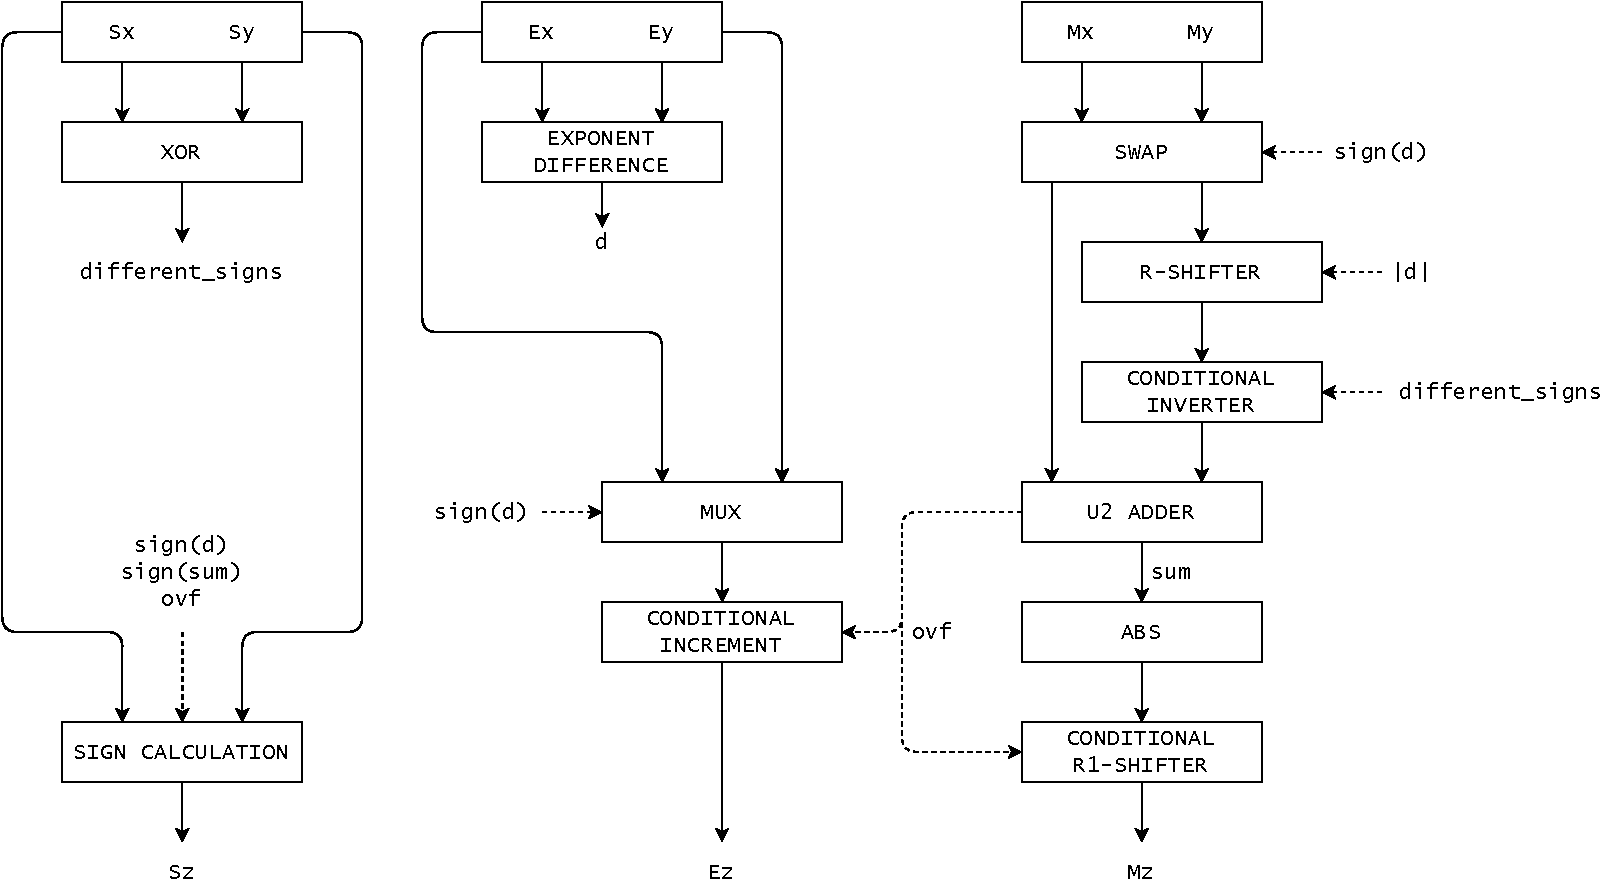
\includegraphics[width=\textwidth]{figures/diagram_add_denorm.pdf}
	\caption{Schemat układu dodawania - zdenormalizowane}
	\label{fig:diagram_add_denorm}
\end{figure}

Na początku układ oblicza różnicę wykładników, żeby następnie wyrównać drugą z nich do tej samej wartości wykładnika.
Liczba z mniejszym wykładnikiem jest przesuwana w prawo o ilość bitów równą wartości różnicy wykładników.
Jeżeli liczby mają różne znaki, to wyrównywana liczba jest dodatkowo negowana.
Umożliwia to sumowanie mantys w U2 wykorzystując obliczony wcześniej bit \texttt{different\_signs} jako przeniesienie wejściowe.
Wewnątrz sumatora wykrywane jest przepełnienie i po obliczeniu wartości bezwzględnej wyniku, wykorzystywane do ewentualnego przesunięcia go w prawo o jeden bit.
W~takim przypadku zwiększany jest też wykładnik wyjściowy.
Wyznaczenie znaku w~przypadku liczb zdenormalizowanych nie jest łatwe.
Wynika to z faktu, że nawet gdy wykładnik jednej z liczb jest większy od drugiej, to różnica w~mantysach może być jeszcze większa.
Wobec tego, konieczne jest wykorzystanie znaków różnicy wykładników, sumy mantys oraz bitu \texttt{ovf} informującym o~przepełnieniu.

Zaimplementowany przez nas układ dodawania liczb znormalizowanych oparty jest o wersję zdenormalizowaną.
Różnice zaznaczyliśmy na rysunku \ref{fig:diagram_add_ieee754} na zielono.

% schemat dodawania IEEE-754
\begin{figure}[H]
	\centering
	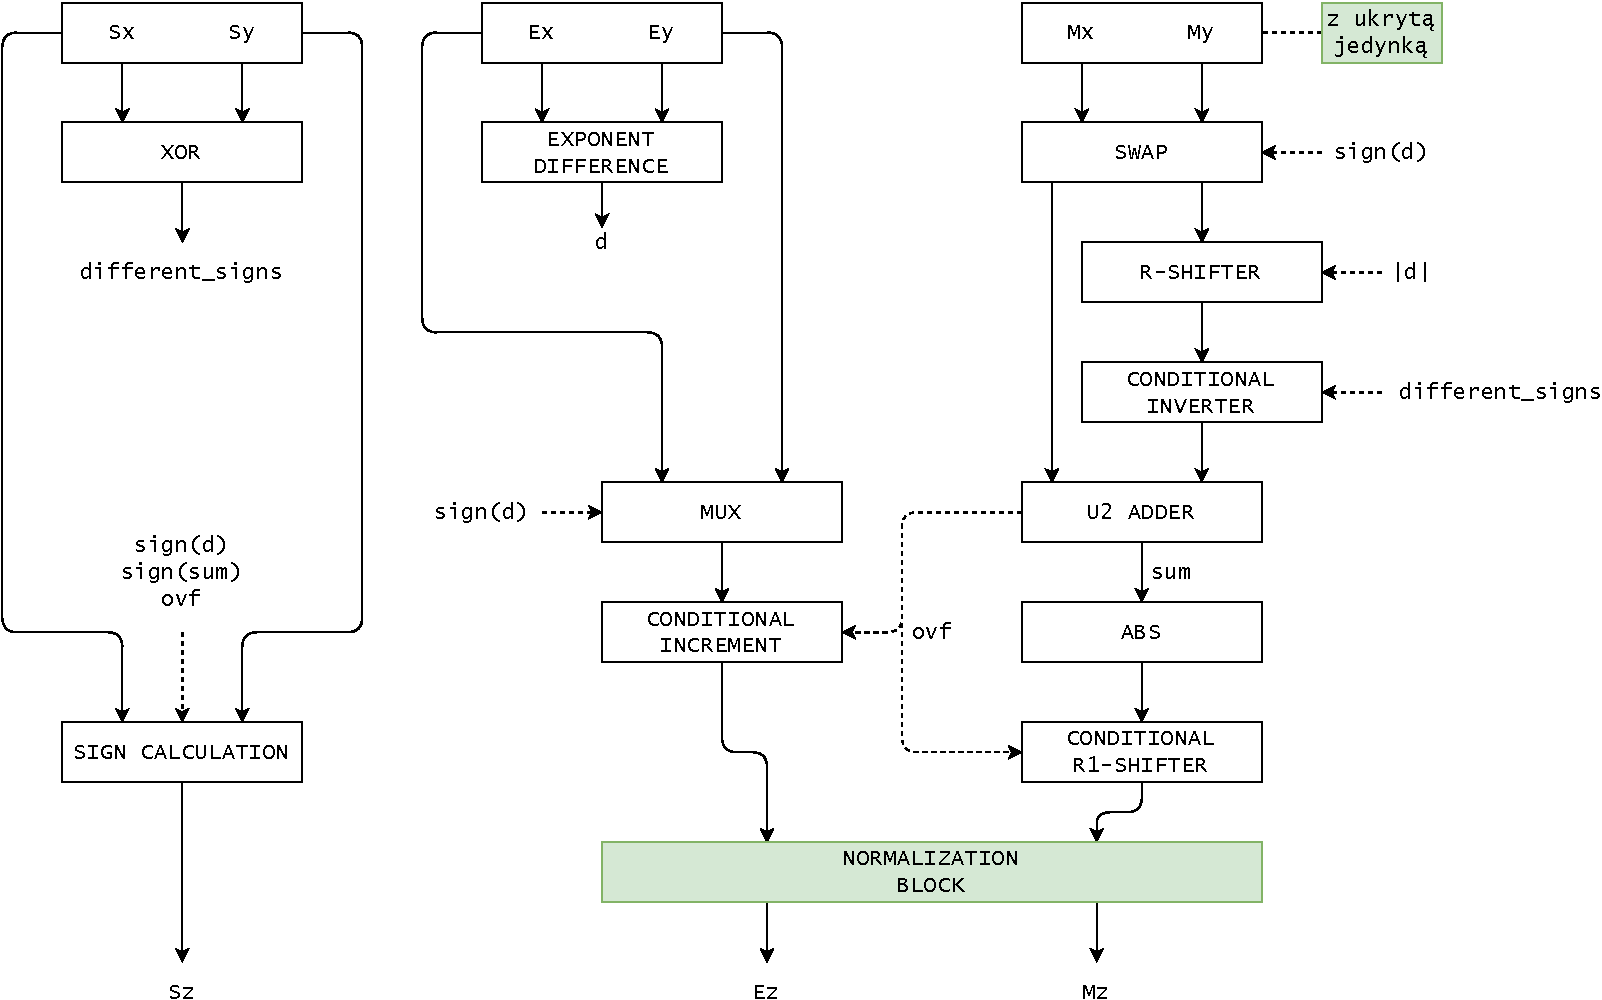
\includegraphics[width=\textwidth]{figures/diagram_add_ieee754.pdf}
	\caption{Schemat układu dodawania - \emph{IEEE-754}}
	\label{fig:diagram_add_ieee754}
\end{figure}

% napisać o znaku
Pierwszą zmianą jest warunkowe dodanie ukrytej jedynki.
Drugą zaznaczoną zmianą jest blok normalizacyjny.
Mantysa jest przesuwana w lewo dopóki na pozycji ukrytego bitu nie pojawi się 1.
Natomiast inną zmianą, która nie jest uwzględniona na schemacie, jest szerokość bitowa sumy mantys.
W wersji liczb znormalizowanych ma ona 48 bitów.

\subsection{Układy mnożenia}

Kolejnym układem, który zaimplementowaliśmy, był układ mnożący, który podobnie jak układ dodawania pochodzi z artykułu \cite{art:old}.
Autorzy nadali mu nazwę \emph{M}.
Jest to pierwsza wersja zaproponowanej przez autorów implementacji układu mnożenia liczb zdenormalizowanych.

% schemat mnożenia zdenormalizowanego
\begin{figure}[H]
	\centering
	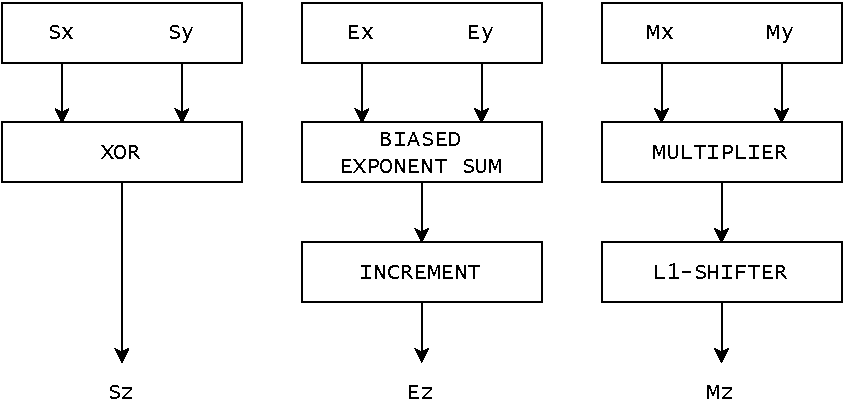
\includegraphics[width=\textwidth]{figures/diagram_mul_denorm.pdf}
	\caption{Schemat układu mnożenia - zdenormalizowane}
	\label{fig:diagram_mul_denorm}
\end{figure}

W przeciwieństwie do sumatora, wyznaczenie znaku jest prostą operacją \texttt{XOR}.
Wykładnik jest sumą wykładników wejściowych z odjętym obciążeniem.
Autorzy przyjęli założenie, że operacja mnożenia mantys, zawsze zakończy się przepełnieniem.
Wobec tego wykładnik wyjściowy jest zawsze zwiększany o jeden, a~mantysa przesuwana w prawo.
W przypadku braku wystąpienia przepełnienia, tracony jest jeden bit precyzji.

Zmiany względem układu mnożącego liczby zgodne ze standardem \emph{IEEE-754} są w tym przypadku niewielkie.

% schemat mnozenia IEEE-754
\begin{figure}[H]
	\centering
	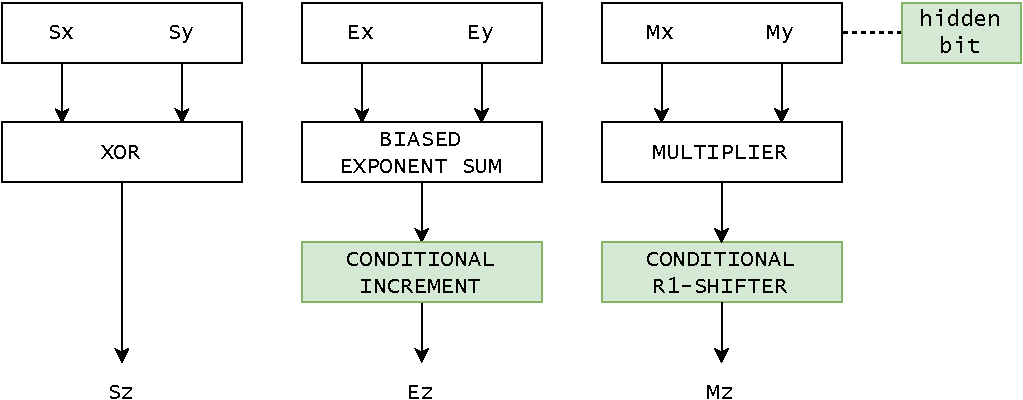
\includegraphics[width=\textwidth]{figures/diagram_mul_ieee754.pdf}
	\caption{Schemat układu mnożenia - \emph{IEEE-754}}
	\label{fig:diagram_mul_ieee754}
\end{figure}

Ponieważ wynik mnożenia dwóch licz znormalizowanych gwarantuje pojawienie się jedynki na jednym z dwóch najstarszych bitów wyniku, normalizacja sprowadza się do warunkowego przesunięcia w prawo w zależności od wystąpienia przepełnienia.


\section{Narzędzia}
Do implementacji układów dodawania i mnożenia użyliśmy języka \emph{Verilog}.
W \emph{C} napisaliśmy funkcje konwertujące wartości typu \texttt{double} na \texttt{float} konieczne do porówania wyników.
\emph{Python} służył jako język, z którego wywoływane były wszystkie polecenia kompilujące wcześniej wspomniane funkcje w \emph{C}, generujące oraz uruchamiające pliki testowe \emph{Veriloga}.
Przy użyciu \emph{Pythona} obliczaliśmy również błędy obliczeniowe wynikające z formatu zdenormalizowanych liczb zmiennoprzecinkowych oraz wykresy je prezentujące.
Do tworzenia wykresów posłużyliśmy się biblioteką \emph{Matplotlib}.
Narzędzie \emph{Icarus Verilog} posłużyło nam do kompilacji i~uruchamiania modułów napisanych w języku \emph{Verilog}.
Natomiast do sprawdzenia poprawności wyników poszczególnych bloków i debugowania programu używaliśmy programu \emph{GTKWave}.
Do utworzenia diagramów została użyta aplikacja \url{diagrams.net}.
Całość kodu była tworzona w programie \emph{Visual Studio Code}.
Testowanie i uruchamianie miało miejsce w systemie Ubuntu na maszynie wirtualnej \emph{WSL 2}.


\section{Opis sposobu testowania}
Stworzone układy sumatora i mnożenia liczb zdenormalizowanych zostały przetestowane pod względem różnic pomiędzy wynikami w swoich odpowiednikach w implementacji \emph{IEEE-754}.
Testowanie rozpoczeliśmy od wygenerowania liczb pseudolosowych w zakresie, w którym zadbaliśmy o to, aby nie doszło do przepełnienia wykładnika.
Wygenerowana liczba utworzona została w języku \emph{Python}, więc była podwójnej precyzji.
Przy pomocy zaimplementowanej przez nas funkcji, zmieniliśmy ją na liczbę pojedynczej precyzji.

Kolejnym krokiem w testowaniu było wykonanie odpowiednich dodawań lub mnożeń w zależności od testowanych układów.
Program następnie startował symulator uruchamiający kolejne układy.
Pierwszym z nich był zaimplementowany przez nas układ działający na liczbach zdenormalizowanych.
Drugim był układ częściowo zgodny ze standardem \emph{IEEE-754}.
Do tego obliczaliśmy wynik operacji na liczbach podwójnej precyzji, którego używaliśmy jako wartości referencyjnej do porównywania wyników.
Tak otrzymane liczby były zapisywane do plików \emph{CSV}.

Testowanie przeprowadzilismy dla następujących ilości wyników 100, 1 000, 10 000, 100 000, 1 000 000, 10 000 000.
Uznaliśmy, że wykresy najlepiej obrazowały otrzymane wyniki przy 1 000 000 punktów.
Możliwe jest wtedy zaobserwowanie szczegółów pozwalających na analizę wyników.
Przy większych ilościach punktów, wykresy stawały się nieczytelne.

Następnym krokiem było porównanie poszczególnych wartości liczb zdenormalizowanych i odpowiadającym im liczb referencyjnych.
Dla każdego wyniku obliczyliśmy błąd względny używając wyniku liczb podwójnej precyzji jako wartości referencyjnej rysunki \ref{fig:add_relative}, \ref{fig:sub_relative}, \ref{fig:mul_relative}.
Dodatkowo utworzyliśmy wykresy prezentujące błąd bezwzględny w ULP - rysunki \ref{fig:add_ulp}, \ref{fig:sub_ulp}, \ref{fig:mul_ulp}.


\section{Wyniki pomiarów}

\begin{figure}[H]
	\centering
	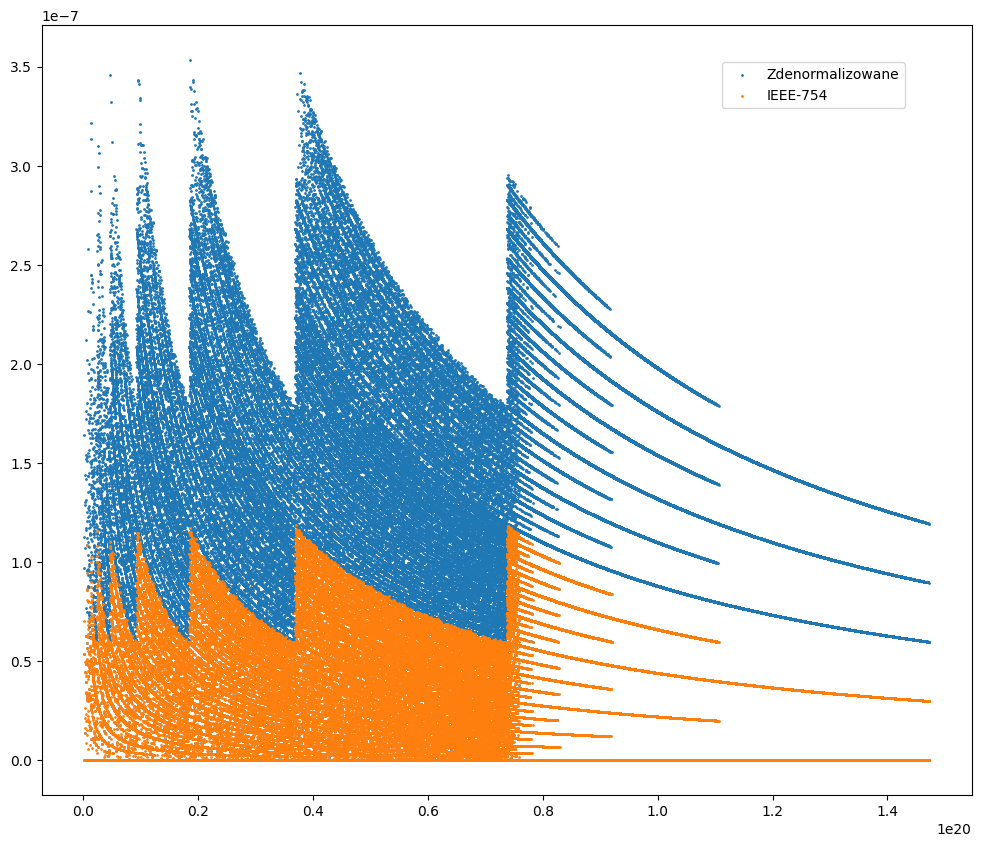
\includegraphics[height=0.4\textheight]{figures/add_relative.png}
	\caption{Błąd względny - dodawanie}
	\label{fig:add_relative}
\end{figure}

\begin{figure}[H]
	\centering
	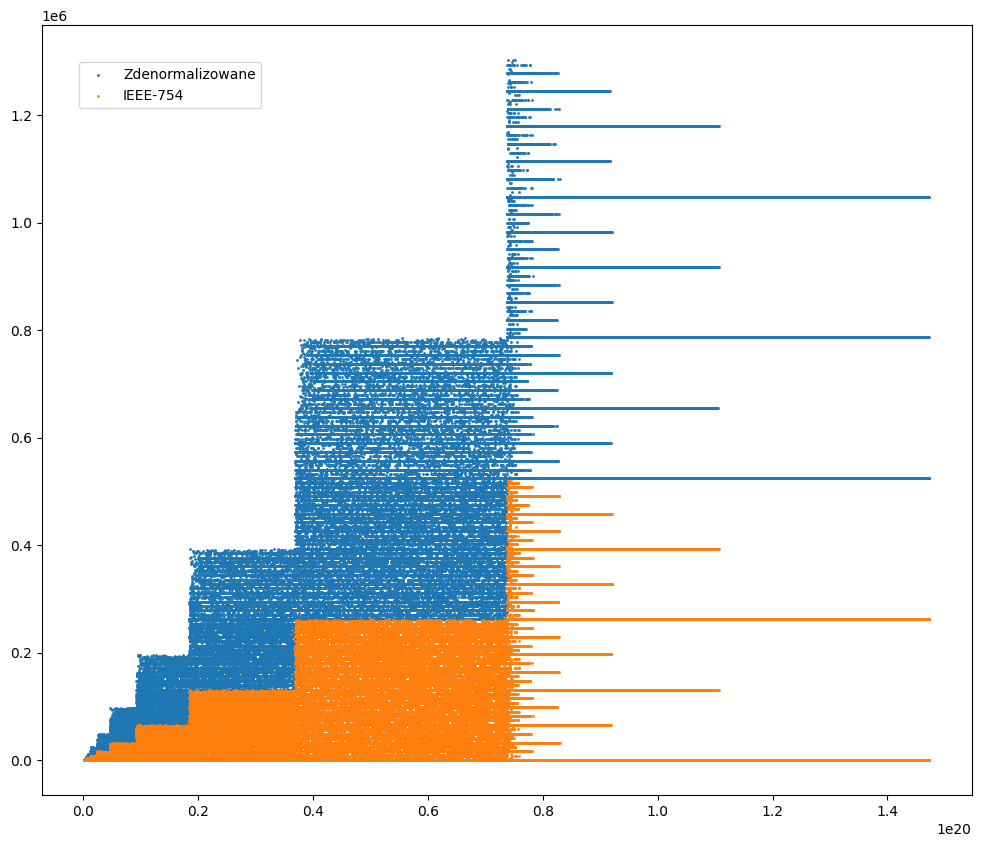
\includegraphics[height=0.4\textheight]{figures/add_ulp.png}
	\caption{Błąd bezwzględny - dodawanie}
	\label{fig:add_ulp}
\end{figure}


\begin{figure}[H]
	\centering
	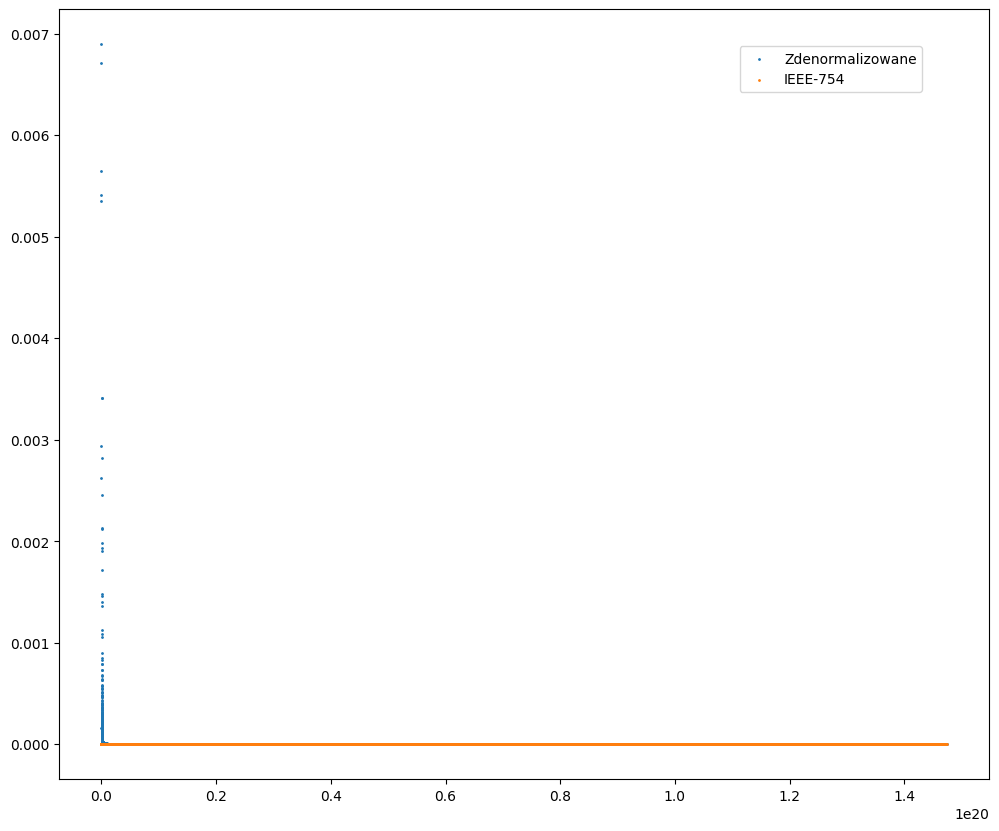
\includegraphics[height=0.4\textheight]{figures/sub_relative.png}
	\caption{Błąd względny - odejmowanie}
	\label{fig:sub_relative}
\end{figure}

\begin{figure}[H]
	\centering
	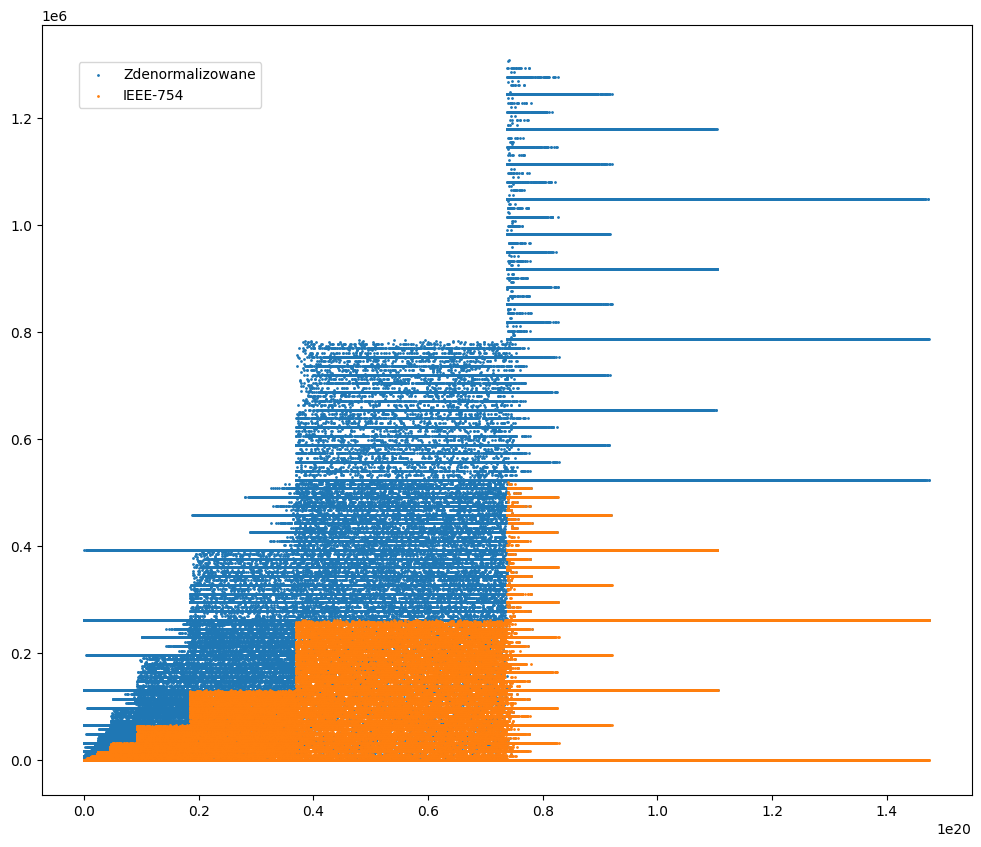
\includegraphics[height=0.4\textheight]{figures/sub_ulp.png}
	\caption{Błąd bezwzględny - odejmowanie}
	\label{fig:sub_ulp}
\end{figure}


\begin{figure}[H]
	\centering
	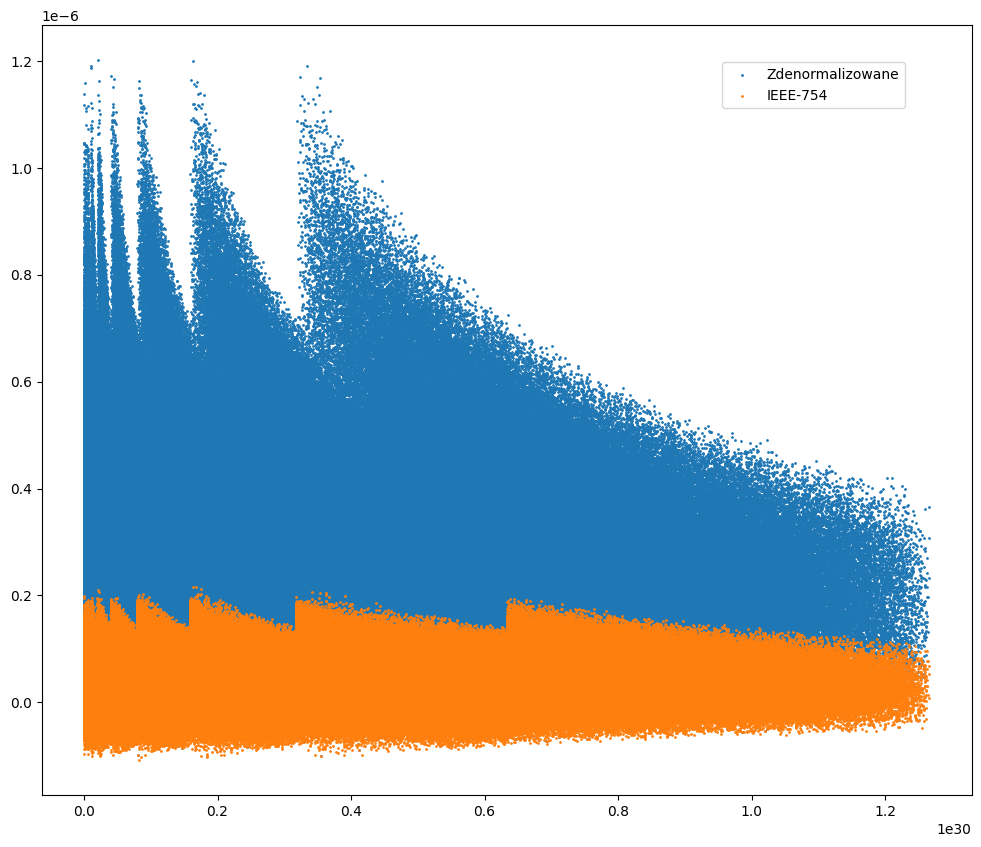
\includegraphics[height=0.4\textheight]{figures/mul_relative.png}
	\caption{Błąd względny - mnożenie}
	\label{fig:mul_relative}
\end{figure}

\begin{figure}[H]
	\centering
	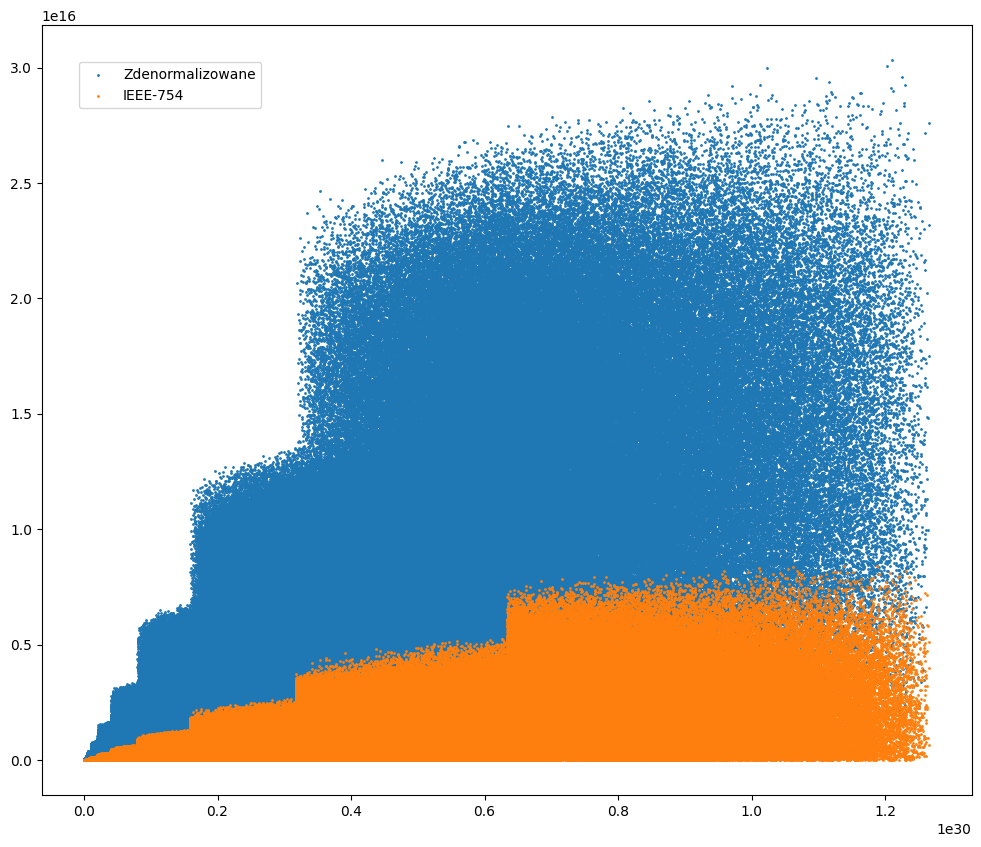
\includegraphics[height=0.4\textheight]{figures/mul_ulp.png}
	\caption{Błąd bezwzględny - mnożenie}
	\label{fig:mul_ulp}
\end{figure}


\section{Wnioski}
% Wyniki naszych badań są trudne do analizowania. 
Podstawową i najbardziej zauważalną różnicą jest wydzielenie się dwóch grup punktów przedstawiających wyniki dla liczb zdenormalizowanych i znormalizowanych.
W pomiarach widzimy różnicę w utracie dokładności poprzez przesunięcie wszystkich bitów w prawo i pozbycie się ukrytego bitu w liczbach zdenormalizowanych.
Różnice w działaniu układów sprawiają, że implementacja dla liczb zdenormalizowanych jest prostsza, zużywa mniej komponentów, a przez to jest mniej energochłonna.

Łatwo zaobserwować linie powstałe na wykresie.
Ich obecność wynika ze stałej liczby bitów reprezentacji liczby.
Ponieważ zbiór liczb możliwych do przedstawienia w każdym z badanych zapisów jest skończony, to wyniki są zaokrąglane, a widoczne linie są tego wynikiem.

% dlatego zaproponowali nowe rozwiązanie \cite{art:new}

% Kolejną różnicą, którą możemy zauważyć na każdym z rysunków jest to, że liczby zdenormalizowane posiadają większe różnicę i są bardziej rozrzucone po całym wykresie.


% ponieważ podczas operacji odejmowania mantysy dążą do zera, to w ieee754 dwukrotnie większa ilość bitów (48) na wynik sprawia, że można wcześniej przesunięte bity "wrócić" podczas normalizacji, gdzie dla zdenormalizowanych nawet, gdyby te bity tam były, to nic by ich nie przesunęło bo nie ma normalizacji


% Na rysunku \ref{fig:add_relative} czy też rysunku \ref{fig:add_ulp}


\newpage
\phantomsection
\addcontentsline{toc}{section}{Literatura}
\bibliography{bibliography}
\bibliographystyle{plabbrv}


\end{document}
